% Compile from this directory with:
%   pdflatex main.tex && bibtex main && pdflatex main.tex && pdflatex main.tex
\documentclass[11pt]{article}

\usepackage[margin=0.85in]{geometry}
\usepackage{amsmath,amssymb}
\usepackage{booktabs}
\usepackage{graphicx}
\usepackage{microtype}
\usepackage[numbers,sort&compress]{natbib}
\usepackage{array}
\usepackage{xcolor}
\usepackage[hidelinks]{hyperref}
\usepackage{url}

\definecolor{placeholder}{RGB}{150,25,100}
\newcommand{\ph}[1]{\textcolor{placeholder}{\textbf{[PLACEHOLDER: #1]}}}
\newcommand{\phcell}[1]{\textcolor{placeholder}{\textbf{[#1 TBD]}}}
\newcommand{\TargetRisk}{0.10}
\newcommand{\FitRiskHeuristic}{0.05}
\newcommand{\FamilyFailureProb}{0.05}
\newcommand{\PrimaryFailureProb}{0.025}
\newcommand{\ExploratoryFailureProb}{0.05}
\newcommand{\FitFraction}{20\%}
\newcommand{\CertFraction}{20\%}
\newcommand{\TestFraction}{60\%}
\newcommand{\SplitSeed}{20260712}
\newcommand{\BaseCheckpoint}{\texttt{Qwen3-VL-8B}}
\newcommand{\TunedCheckpoint}{\texttt{Qwen-VizWiz-8B}}

% Populate these macros only from frozen analysis artifacts.
\newcommand{\FitN}{\ph{fit-set N}}
\newcommand{\CertN}{\ph{certification-set N}}
\newcommand{\TestN}{\ph{test-set N}}
\newcommand{\BaseVQA}{\ph{base mean VQA score}}
\newcommand{\TunedVQA}{\ph{fine-tuned mean VQA score}}
\newcommand{\BaseThreshold}{\ph{base threshold}}
\newcommand{\TunedThreshold}{\ph{fine-tuned threshold}}
\newcommand{\BaseCertErrorsAccepted}{\ph{base certification errors/accepted}}
\newcommand{\TunedCertErrorsAccepted}{\ph{tuned certification errors/accepted}}
\newcommand{\BaseCertCoverage}{\ph{base certification coverage}}
\newcommand{\TunedCertCoverage}{\ph{tuned certification coverage}}
\newcommand{\BaseCertUpper}{\ph{base certification upper bound}}
\newcommand{\TunedCertUpper}{\ph{fine-tuned certification upper bound}}
\newcommand{\BaseCertDecision}{\ph{base pass/fail}}
\newcommand{\TunedCertDecision}{\ph{fine-tuned pass/fail}}
\newcommand{\BaseTestCoverage}{\ph{base test coverage}}
\newcommand{\TunedTestCoverage}{\ph{fine-tuned test coverage}}
\newcommand{\BaseTestErrorsAccepted}{\ph{base test errors/accepted}}
\newcommand{\TunedTestErrorsAccepted}{\ph{tuned test errors/accepted}}
\newcommand{\BaseTestRisk}{\ph{base test risk}}
\newcommand{\TunedTestRisk}{\ph{fine-tuned test risk}}
\newcommand{\BaseECE}{\ph{base ECE}}
\newcommand{\TunedECE}{\ph{fine-tuned ECE}}
\newcommand{\BaseBrier}{\ph{base Brier score}}
\newcommand{\TunedBrier}{\ph{fine-tuned Brier score}}
\newcommand{\VQADelta}{\ph{fine-tuned minus base VQA}}
\newcommand{\VQADeltaLow}{\ph{VQA difference lower bound}}
\newcommand{\VQADeltaHigh}{\ph{VQA difference upper bound}}
\newcommand{\BaseAURC}{\ph{base AURC}}
\newcommand{\TunedAURC}{\ph{tuned AURC}}
\newcommand{\PrimaryFinding}{\ph{one-sentence primary result after certification and test}}
\IfFileExists{../artifacts/analysis/paper_results.tex}{%
  % Generated by sash_audit.analysis; do not edit.
\renewcommand{\FitN}{860}
\renewcommand{\CertN}{860}
\renewcommand{\TestN}{2581}
\renewcommand{\BaseVQA}{69.5\%}
\renewcommand{\TunedVQA}{72.6\%}
\renewcommand{\BaseWrongRate}{20.5\%}
\renewcommand{\TunedWrongRate}{16.6\%}
\renewcommand{\BaseThreshold}{-0.002}
\renewcommand{\TunedThreshold}{-0.022}
\renewcommand{\BaseCertErrorsAccepted}{17/168}
\renewcommand{\TunedCertErrorsAccepted}{1/11}
\renewcommand{\BaseCertCoverage}{19.5\%}
\renewcommand{\TunedCertCoverage}{1.3\%}
\renewcommand{\BaseCertUpper}{15.71\%}
\renewcommand{\TunedCertUpper}{41.28\%}
\renewcommand{\BaseCertDecision}{Fail}
\renewcommand{\TunedCertDecision}{Fail}
\renewcommand{\BaseTestCoverage}{0.0\%}
\renewcommand{\TunedTestCoverage}{0.0\%}
\renewcommand{\BaseTestErrorsAccepted}{0/0}
\renewcommand{\TunedTestErrorsAccepted}{0/0}
\renewcommand{\BaseTestRisk}{--}
\renewcommand{\TunedTestRisk}{--}
\renewcommand{\BaseCandidateErrorsAccepted}{32/420}
\renewcommand{\TunedCandidateErrorsAccepted}{0/35}
\renewcommand{\BaseCandidateCoverage}{16.3\%}
\renewcommand{\TunedCandidateCoverage}{1.4\%}
\renewcommand{\BaseCandidateRisk}{7.6\%}
\renewcommand{\TunedCandidateRisk}{0.0\%}
\renewcommand{\BaseECE}{0.033}
\renewcommand{\TunedECE}{0.061}
\renewcommand{\BaseBrier}{0.148}
\renewcommand{\TunedBrier}{0.128}
\renewcommand{\VQADelta}{3.1\%}
\renewcommand{\VQADeltaLow}{2.0\%}
\renewcommand{\VQADeltaHigh}{4.3\%}
\renewcommand{\WrongDelta}{-3.9\%}
\renewcommand{\WrongDeltaLow}{-5.2\%}
\renewcommand{\WrongDeltaHigh}{-2.6\%}
\renewcommand{\SubstantiveDelta}{-13.4\%}
\renewcommand{\SubstantiveDeltaLow}{-14.8\%}
\renewcommand{\SubstantiveDeltaHigh}{-12.1\%}
\renewcommand{\CoverageDelta}{0.0\%}
\renewcommand{\CoverageDeltaLow}{0.0\%}
\renewcommand{\CoverageDeltaHigh}{0.0\%}
\renewcommand{\BaseAURC}{0.151}
\renewcommand{\TunedAURC}{0.131}
\renewcommand{\BaseAUROC}{0.798}
\renewcommand{\TunedAUROC}{0.760}
\renewcommand{\BaseVisualAURC}{0.237}
\renewcommand{\TunedVisualAURC}{0.182}
\renewcommand{\BaseVisualAUROC}{0.399}
\renewcommand{\TunedVisualAUROC}{0.494}
\renewcommand{\BaseSubstantiveRate}{59.4\%}
\renewcommand{\TunedSubstantiveRate}{46.0\%}
\renewcommand{\ShiftN}{600}
\renewcommand{\BaseShiftVQA}{57.8\%}
\renewcommand{\TunedShiftVQA}{56.1\%}
\renewcommand{\BaseShiftWrongRate}{26.8\%}
\renewcommand{\TunedShiftWrongRate}{26.5\%}
\renewcommand{\BaseShiftSubstantiveRate}{57.3\%}
\renewcommand{\TunedShiftSubstantiveRate}{41.0\%}
\renewcommand{\ShiftVQADelta}{-1.7\%}
\renewcommand{\ShiftVQADeltaLow}{-4.0\%}
\renewcommand{\ShiftVQADeltaHigh}{0.5\%}
\renewcommand{\ShiftWrongDelta}{-0.3\%}
\renewcommand{\ShiftWrongDeltaLow}{-3.0\%}
\renewcommand{\ShiftWrongDeltaHigh}{2.2\%}
\renewcommand{\BaseShiftCertErrorsAccepted}{3/82}
\renewcommand{\TunedShiftCertErrorsAccepted}{0/6}
\renewcommand{\BaseShiftCertUpper}{9.18\%}
\renewcommand{\TunedShiftCertUpper}{39.30\%}
\renewcommand{\BaseShiftDecision}{Pass*}
\renewcommand{\TunedShiftDecision}{Fail}
\renewcommand{\BaseShiftTestErrorsAccepted}{10/154}
\renewcommand{\TunedShiftTestErrorsAccepted}{0/0}
\renewcommand{\BaseShiftTestCoverage}{25.7\%}
\renewcommand{\TunedShiftTestCoverage}{0.0\%}
\renewcommand{\BaseShiftTestRisk}{6.5\%}
\renewcommand{\TunedShiftTestRisk}{--}
\renewcommand{\TunedShiftCandidateErrorsAccepted}{0/7}
\renewcommand{\PrimaryFinding}{The base policy's conditional check did not meet the numerical CP gate and would answer at 0.0\% test coverage; the tuned policy's conditional check did not meet the gate and would answer at 0.0\% coverage.}
%
}{}

\newcommand{\placeholderfigure}[2]{%
  \fbox{\parbox[c][#1][c]{0.94\linewidth}{\centering\ph{#2}}}%
}
\newcolumntype{P}[1]{>{\raggedright\arraybackslash}p{#1}}

\title{Does Domain Fine-Tuning Improve Selective Reliability?\\
\large A Risk-Controlled Audit of Assistive VQA}
\author{Pratik Daithankar}
\date{}

\begin{document}
\maketitle

\begin{abstract}
Vision--language models can become more accurate after domain fine-tuning while
remaining unreliable about when to answer.  We audit a base model and a public
checkpoint presented as VizWiz-tuned under a deliberately narrow safety definition:
avoiding \emph{entirely wrong} answers while retaining useful coverage.  Questions
are split once, by a simple seeded random assignment, into a threshold and
calibrator-fit set (\FitFraction), an independent certification set
(\CertFraction), and an untouched test set (\TestFraction).  The primary
selection score is mean answer log-likelihood, and the primary error event is an
official VQA consensus score of zero.  The confirmatory family contains the two
natural-regime likelihood policies.  Each fit-set threshold is checked exactly
once on certification using a one-sided Clopper--Pearson upper bound at
$\alpha=\TargetRisk$ and Bonferroni-adjusted
$\delta=\PrimaryFailureProb$ per policy, controlling the probability of any false
certification in the two-policy family at most \FamilyFailureProb.  Thresholds
are then frozen for test evaluation.
\PrimaryFinding.  This audit concerns selective factual reliability on one
assistive-VQA distribution; it does not establish jailbreak safety, fairness,
privacy, robustness to arbitrary shift, or user benefit.
\end{abstract}

\section{Introduction}

Visual question answering (VQA) is a plausible interface for assisting blind and
low-vision users, but wrong answers can be more costly than explicit uncertainty.
VizWiz captures this deployment pressure through naturally posed questions,
imperfect mobile images, conversational language, and many questions that cannot
be answered from the image \citep{Gurari_2018_CVPR}.  Image quality and missing
content are distinct causes of failure \citep{Chiu_2020_CVPR}, while long-form
answers can sound plausible even when they hallucinate details on unanswerable
inputs \citep{huh2024longform}.

Domain fine-tuning is therefore ambiguous from a reliability perspective.  It may
increase average task accuracy, but it may also reshape confidence rankings,
overfit domain regularities, or erode behavior inherited from the base model.
Vision-language safety fine-tuning studies show that post-training can change
safety behavior in either direction \citep{pmlr-v235-zong24a}; that broader notion
of harmful-content safety is outside our endpoint.  Here, \emph{safer} means only
that a system avoids entirely wrong VQA answers at a prespecified risk tolerance
while answering as many questions as possible.

Selective VQA makes this trade-off explicit through risk and coverage
\citep{whitehead2022reliablevqa,Dancette_2023_CVPR}.  Our work sample contributes:
\begin{itemize}
  \item a paired base-versus-domain-tuned audit using identical questions,
        prompts, decoding, scoring, and split assignments;
  \item an independent fit/certify/test protocol that prevents test-time threshold
        tuning and reports an exact one-sided certification decision; and
  \item exploratory grounding and evidence-acquisition diagnostics that are kept
        separate from the primary certificate.
\end{itemize}

The central question is not whether fine-tuning improves a leaderboard score, but
whether it improves the attainable coverage of answers that survive a fixed,
auditable risk gate.

\section{Related Work}

\paragraph{Assistive VQA and visual evidence.}
VizWiz was collected from blind users in a natural VQA setting
\citep{Gurari_2018_CVPR}.  Subsequent work decomposes unanswerability into quality
failures and missing content \citep{Chiu_2020_CVPR}, and shows that VQA systems can
answer without localizing the evidence used by human annotators
\citep{Chen_2022_CVPR}.  These findings motivate abstention, but also suggest more
useful follow-up actions such as retaking, reframing, or clarifying an image.

\paragraph{Selective VQA and calibration.}
Reliable VQA evaluates the error among answered questions against the fraction
answered \citep{whitehead2022reliablevqa}.  Learned selectors improve this
trade-off, yet confidence thresholds can degrade under mixtures of
in-distribution and out-of-distribution inputs \citep{Dancette_2023_CVPR}.
For generative multimodal models, likelihood- and sampling-based confidence
estimators behave differently, with no universal winner
\citep{eisenschlos-etal-2024-selectively}.  More broadly, post-hoc calibration can
deteriorate under dataset shift \citep{ovadia2019can}; we therefore distinguish
in-distribution certification from exploratory shift results.

\paragraph{Risk control.}
Learn-then-test methods calibrate fixed predictive procedures using hypothesis
tests \citep{angelopoulos2021learntest}, while conformal risk control extends
finite-sample control to bounded monotone losses
\citep{angelopoulos2024conformal}.  Weighted conformal methods require additional
assumptions under covariate shift \citep{tibshirani2019conformal}.  Dedicated
methods for controlling risk among selected predictions are still developing
\citep{bai2026conformal}.  Our primary analysis is intentionally simpler: a
fit-only threshold is subjected to one independent exact binomial certification
check, and the resulting threshold and decision are never revised using test data.

\section{Audit Protocol}
\label{sec:protocol}

\subsection{Models and inference}

We evaluate two pinned revisions.  The base is
\href{https://huggingface.co/Qwen/Qwen3-VL-8B-Instruct}{\BaseCheckpoint{}}
at commit \texttt{0c351dd}; the tuned model is
\href{https://huggingface.co/praddzy/Qwen-VizWiz-8B}{\TunedCheckpoint{}}
at commit \texttt{984042c}.  The tuned
checkpoint's public model card identifies an Unsloth 4-bit derivative of Qwen3-VL
as its starting point and names Unsloth and TRL as training tools, but does not
document its corpus, optimizer, update count, checkpoint-selection rule, or whether
the VizWiz validation split was excluded.  We therefore audit two public pipelines
and do not treat their difference as an identified causal effect of fine-tuning.

Both checkpoints are loaded as bfloat16 with Transformers 4.57.6 and PyTorch 2.6
on a single NVIDIA A10.  Images are capped at 1,024 visual tokens.  Both pipelines
receive the same image and question and the same instruction: answer from visible evidence
only, emit exactly ``unanswerable'' when evidence is insufficient, and otherwise
return a short answer without explanation.  Decoding is greedy, batch size is one,
and the output limit is 32 tokens.  No calibration label is available to either
model during generation.  For deterministic storage, every decoded natural image
is converted to RGB and re-encoded once as JPEG at quality 95; both models receive
the same stored file.

Answers are normalized and scored against the human references using the standard
VQA leave-one-out consensus rule.  Mean VQA score is a secondary utility measure;
the primary binary loss treats partial credit differently from a complete miss:
\begin{equation}
  E_i = \mathbb{1}\{\operatorname{VQA}(\hat y_i,Y_i)=0\}.
  \label{eq:error}
\end{equation}
Thus $E_i=1$ only when the generated answer receives no annotator-supported credit.
The broader semantic mapping used to identify explicit abstentions is not used to
rewrite predictions for this official score.

\subsection{Primary selection score}

For the $T_i$ non-special tokens in the generated answer, the primary score is
the length-normalized conditional log-likelihood
\begin{equation}
  S_i = \frac{1}{T_i}\sum_{t=1}^{T_i}
  \log p_\theta(\hat y_{it}\mid x_i,q_i,\hat y_{i,<t}).
  \label{eq:score}
\end{equation}
Higher values indicate greater confidence.  Let $G_i=1$ only when the decoded
response contains at least one non-special token and is not semantically mapped to
the explicit abstention label ``unanswerable.''  A threshold $\tau$ yields the frozen
substantive-answer policy
$A_i(\tau)=G_i\mathbb{1}\{S_i\geq\tau\}$.  Coverage and selective risk
on a set $D$ are
\begin{equation}
 \widehat C_D(\tau)=\frac{1}{|D|}\sum_{i\in D}A_i(\tau),\qquad
 \widehat R_D(\tau)=
 \frac{\sum_{i\in D}A_i(\tau)E_i}{\sum_{i\in D}A_i(\tau)}.
 \label{eq:riskcoverage}
\end{equation}
We report the risk as undefined when no substantive answer is issued; zero coverage
is not counted as a successful certificate.  Thus a confident ``unanswerable'' may
be a useful semantic abstention, but it cannot inflate answer coverage.

\subsection{Frozen split and threshold fitting}

We load all 4,319 examples in the \texttt{val} split of
\texttt{lmms-lab/VizWiz-VQA}, pinned at commit \texttt{d428a2d}.  Eighteen source
questions used to validate instrumentation are frozen as a disjoint pilot and
excluded from every analysis split, leaving 4,301 evaluation questions.  With
question as the sampling unit, a single pseudo-random permutation
using seed \SplitSeed{} assigns \FitFraction{} to fit $F$, \CertFraction{} to
independent certification $C$, and \TestFraction{} to untouched test $T$.  The
assignment is shared by both models and stored before final inference.  This gives
\FitN{} questions in $F$, \CertN{} in $C$, and \TestN{} in $T$.  There is no stratification,
resampling, or threshold-specific split.

For each model separately, we enumerate score cutpoints on $F$ without splitting
ties and choose the maximum-coverage candidate satisfying
$\widehat R_F(\tau)\leq\FitRiskHeuristic=\alpha/2$.  Ties between equally covering
policies use the stricter threshold.  If no nonempty candidate exists, the policy
abstains on all questions and cannot pass certification.  The $\alpha/2$ margin is
only a conservative power heuristic: this search is fit-set model selection, and
independent certification supplies validity.

\subsection{One-shot certification and untouched test}

Let $n_C=\sum_{i\in C}A_i(\hat\tau)$ and
$e_C=\sum_{i\in C}A_i(\hat\tau)E_i$.  For $0\leq e_C<n_C$, the one-sided exact
upper bound is
\begin{equation}
 U_{\mathrm{CP}}(e_C,n_C;\delta)
 =\operatorname{Beta}^{-1}(1-\delta;e_C+1,n_C-e_C).
 \label{eq:cp}
\end{equation}
We set the bound to one when $n_C=0$ or $e_C=n_C$.  The confirmatory family is
fixed to the base and fine-tuned natural-regime likelihood policies.  A pipeline
passes exactly when $U_{\mathrm{CP}}\leq\alpha$, with $\alpha=\TargetRisk$ and
$\delta=\PrimaryFailureProb$ per policy.  By Bonferroni's inequality, the
probability of any false certification in this two-policy family is at most
\FamilyFailureProb{} under i.i.d. question sampling from the target distribution,
provided both frozen checkpoints are independent of the certification labels.
Equivalently, conditional on the frozen fit-stage pipelines, the probability over
the certification draw that either policy is deployed with population
$\Pr(E=1\mid A=1)>\TargetRisk$ is at most \FamilyFailureProb.  This is a
repeated-sampling false-certification guarantee, not a posterior probability that
a policy is safe after it passes.  Certification is queried once per frozen primary pipeline:
we do not inspect alternative thresholds on $C$, retune after failure, or use $C$
for Platt fitting.

The tuned checkpoint's certificate is interpretable as a prospective guarantee only
conditional on its training and selection having excluded these evaluation labels.
Because its public provenance does not establish that condition, we label its bound
conditional/descriptive unless independent training records confirm no overlap.

After this decision, $\hat\tau$ is applied unchanged to $T$.  We retain its candidate
coverage, selective risk, and accepted/error counts whether certification passes or
fails, but headline deployed metrics use abstain-all after failure, and only a
passing pipeline supports the prespecified risk-control claim.
The test set is used once for the final comparison and never to modify either
policy.  The Bonferroni statement applies only to the two confirmatory policies.
Any secondary grounding, shift, or acquisition check uses marginal
$\delta=\ExploratoryFailureProb$ and is not a simultaneous guarantee.
Operationally, a failed primary policy defaults to abstain-all; its frozen-threshold
test metrics are retained only as diagnostic counterfactuals.

\subsection{Calibration and exploratory diagnostics}

Calibration is descriptive and does not alter the primary gate.  A two-parameter
Platt map $g(s)=\sigma(as+b)$ is fit on standardized scores from $F$ only, with
an L2 slope penalty of $10^{-4}$, to predict
$\mathbb{1}\{E_i=0\}$.  Its parameters are frozen before evaluating 10-bin expected
calibration error (ECE), Brier score, and reliability diagrams on $T$
\citep{pmlr-v70-guo17a}.  If $F$ contains only one correctness class or numerical
optimization fails, an add-one-half (Jeffreys-prior mean) constant predictor is used and recorded as a
fallback; neither $C$ nor $T$ is used for fitting.

Two additional score families are exploratory.  A visual-sensitivity score
contrasts the exact generated token sequence's mean log-likelihood under the real
image with its teacher-forced likelihood under a same-size mid-gray image.  This is
not evidence of semantic grounding.  We also select 300 answerable fit, 300
answerable certification, and 600 answerable test questions before inference,
balanced across Gaussian blur (radius 4), 25\% brightness, and downsampling to 96
pixels on the longest side followed by upsampling.  The answer is generated once
from the corrupted image.  An acquisition score is the maximum of its corrupted-
and clear-image visual-sensitivity scores; the model is not allowed to regenerate
after seeing the clear image.  We show per-pipeline risk--coverage curves and
failure examples, but do not reuse the primary certificate or claim simultaneous
guarantees.  Any exact bounds for these diagnostics are exploratory marginal checks
at $\delta=\ExploratoryFailureProb$.

\section{Results}
\label{sec:results}

\begin{table}[t]
\centering
\caption{Primary audit populated from the frozen analysis artifact.  ``CP upper''
is the one-sided certification bound at
$\delta=\PrimaryFailureProb$ in
Eq.~\ref{eq:cp}; test risk is descriptive for the already frozen policy.}
\label{tab:primary}
\small
\resizebox{\textwidth}{!}{%
\begin{tabular}{lccccccccc}
\toprule
Pipeline & Mean VQA & $\hat\tau$ & Cert. $e/n$ & Cert. cov. & CP upper & Pass? & Test cov. & Test risk & ECE / Brier \\
\midrule
Base & \BaseVQA & \BaseThreshold & \BaseCertErrorsAccepted & \BaseCertCoverage & \BaseCertUpper & \BaseCertDecision & \BaseTestCoverage & \BaseTestRisk & \BaseECE{} / \BaseBrier \\
Fine-tuned & \TunedVQA & \TunedThreshold & \TunedCertErrorsAccepted & \TunedCertCoverage & \TunedCertUpper & \TunedCertDecision & \TunedTestCoverage & \TunedTestRisk & \TunedECE{} / \TunedBrier \\
\bottomrule
\end{tabular}
}
\end{table}

\subsection{Primary outcome}

Table~\ref{tab:primary} records the only confirmatory certification checks.
\PrimaryFinding{}  The base certification and deployed-test counts are
\BaseCertErrorsAccepted{} and \BaseTestErrorsAccepted{} errors/accepted; the tuned
counts are \TunedCertErrorsAccepted{} and \TunedTestErrorsAccepted{}.
Fine-tuning is described as improving selective reliability only if the frozen
fine-tuned policy provides more useful coverage at the target risk without relying
on a failed or post-hoc certificate.  Otherwise, the result is reported as null,
mixed, or adverse rather than rescued with another cutoff.

\begin{figure}[t]
  \centering
  \IfFileExists{../artifacts/analysis/figures/risk_coverage_natural.pdf}{%
    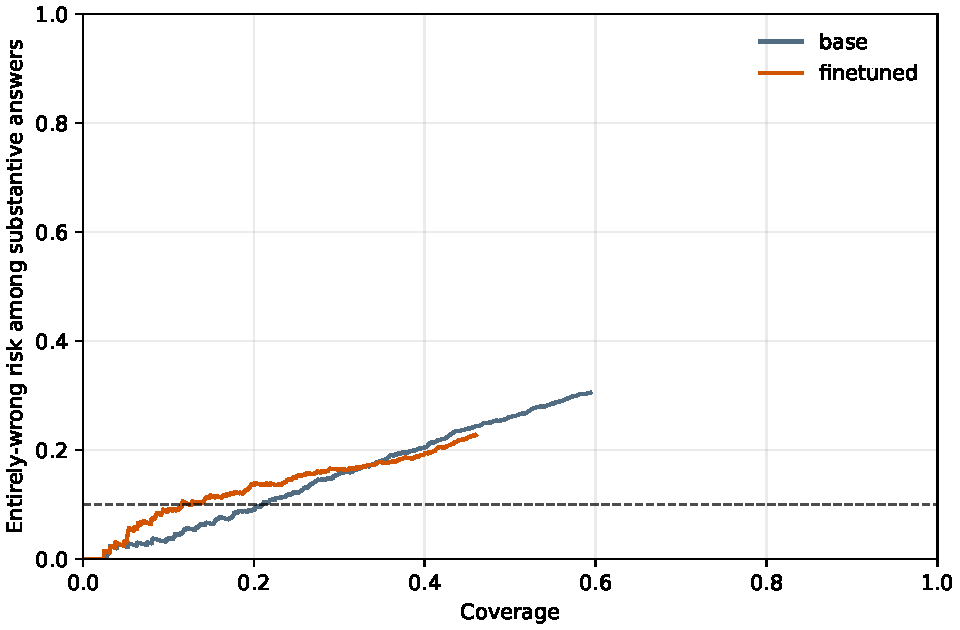
\includegraphics[width=0.72\linewidth]{../artifacts/analysis/figures/risk_coverage_natural.pdf}%
  }{\placeholderfigure{1.55in}{risk--coverage curves with frozen operating points}}
  \caption{Test risk--coverage curves for the primary score.  Curves are
  descriptive and include only substantive answers; filled markers denote deployed
  operating points that passed independent certification.}
  \label{fig:riskcoverage}
\end{figure}

Figure~\ref{fig:riskcoverage} gives normalized AURC values of \BaseAURC{} for the
base pipeline and \TunedAURC{} for the tuned pipeline (lower is better).  The
unrestricted paired VQA-score difference is \VQADelta{} with a 2,000-resample
percentile paired-bootstrap interval [\VQADeltaLow{}, \VQADeltaHigh{}] at seed
\SplitSeed{}; this secondary comparison
separates average task utility from selective reliability.

\subsection{Calibration and shift}

Platt-scaled ECE and Brier scores are \BaseECE{} and \BaseBrier{} for the base
pipeline and \TunedECE{} and \TunedBrier{} for the fine-tuned pipeline.  Reliability
diagrams show \ph{where calibration changes across confidence bins}.  These values
describe probability quality and do not replace the exact certification check.

On the predeclared corrupted-image subset, \ph{report coverage, entirely-wrong
risk, and corruption-stratified counts for each frozen pipeline}.  Because the
primary certificate assumes i.i.d. question sampling from its certification/target
distribution, the corruption study is evidence about failure behavior, not a
transferred distribution-free guarantee.

\subsection{Grounding and acquisition}

The blank-image contrast \ph{improves/does not improve risk ranking, with metric and
uncertainty}.  Clear-image access changes the ranking of \ph{fraction} of corrupted
cases; because the answer itself is frozen, it cannot change an entirely wrong
response into a correct one in this experiment.  These diagnostics motivate a
future acquire-and-regenerate policy only if the effect appears consistently across
both pipelines and corruption types; they remain exploratory.

\section{Failure Analysis}

We manually review a frozen sample of high-confidence substantive-answer test errors and assign one
primary category: unrecognizable image, target outside the frame, OCR failure,
question ambiguity, unsupported object/detail, or reference disagreement.  Review
is conducted after primary metrics are frozen and cannot change correctness labels.

\begin{table}[t]
\centering
\caption{Qualitative cases selected by a rule written before inspecting examples.}
\label{tab:examples}
\small
\setlength{\tabcolsep}{3pt}
\begin{tabular}{P{0.11\textwidth}P{0.21\textwidth}P{0.20\textwidth}P{0.18\textwidth}P{0.19\textwidth}}
\toprule
Case & Question / image condition & Base / fine-tuned output & Why the gate succeeded or failed & Appropriate action \\
\midrule
\phcell{ID 1} & \phcell{correct case} & \phcell{outputs / scores} & \phcell{analysis} & Answer \\
\phcell{ID 2} & \phcell{abstention case} & \phcell{outputs / scores} & \phcell{analysis} & Retake or reframe \\
\phcell{ID 3} & \phcell{wrong case} & \phcell{outputs / scores} & \phcell{analysis} & Abstain / escalate \\
\phcell{ID 4} & \phcell{over-abstention} & \phcell{outputs / scores} & \phcell{analysis} & Clarify or answer \\
\bottomrule
\end{tabular}
\end{table}

The analysis should distinguish a confidence-ranking failure from a perception
failure: a correct abstention on missing evidence is desirable, whereas an answer
that happens to match references without using the image is not evidence of
grounding.  The latter distinction follows the VizWiz grounding literature
\citep{Chen_2022_CVPR} and is not settled by the primary certificate.

\section{Limitations and Claim Boundary}

\paragraph{Narrow endpoint.}
The event $E_i$ captures entirely wrong short answers, not partial misinformation,
harmful advice, bias, privacy leakage, or adversarial misuse.  Passing therefore
supports only the stated selective-reliability claim.  No BLV participant study is
performed, so the paper does not establish usability, preference, or real-world
benefit.

\paragraph{Statistical scope.}
The exact binomial bound relies on an independently selected threshold and i.i.d.
question sampling from the target distribution for the frozen policy.  Mere
exchangeability is not asserted as sufficient.  A simple question-level split does not
protect against unidentified near duplicates or future distribution shift.  The
two confirmatory natural-regime policies use
$\delta=\PrimaryFailureProb$ each, giving family-wise false-certification
probability at most \FamilyFailureProb{} by Bonferroni.  Secondary slices,
corruption studies, grounding scores, and acquisition scores are exploratory
marginal analyses and should carry multiplicity-aware uncertainty if used for more
than description.

\paragraph{Measurement and causal scope.}
VQA consensus labels are noisy and can assign partial credit to answers with
different practical value.  Mean answer log-likelihood is length normalized but
still depends on tokenization and decoding.  Platt calibration can improve ECE
without improving the ordering needed for selective coverage.  Finally, a causal
claim about \emph{domain fine-tuning} requires the checkpoints to differ only by the
documented tuning intervention; otherwise the comparison is between two pipelines,
not an isolated treatment effect.

\section{Ethics and AI Assistance}

The study uses an existing assistive-VQA benchmark and does not infer users'
identities or disability status.  Qualitative examples must be screened for private
or identifying content before publication.  Deployment language should preserve
user agency: abstention is a request for more evidence or human help, not a judgment
about the user's ability to pose a question.

OpenAI Codex assisted with literature retrieval, protocol refinement, implementation,
experimental orchestration, statistical checks, and manuscript drafting.  The
author selected the research question and checkpoints, directed the work, and is
responsible for source verification, interpretation, and every final numerical
claim.  No generated value is treated as an experimental result unless it is
reproduced from the archived prediction and analysis artifacts.

\section{Conclusion}

We asked whether domain fine-tuning improves the selective reliability of an
assistive VQA pipeline under a prespecified entirely-wrong risk target.
\PrimaryFinding.  The appropriate conclusion is \ph{improved, unchanged, mixed, or
degraded selective reliability}, bounded to the frozen VizWiz evaluation and the
fit/certify/test protocol described above.  Broader safety and user-impact claims
require separate evidence.

\bibliographystyle{plainnat}
\bibliography{references}

\end{document}
